\chapter{Einleitung}
\section{Ausgangssituation}
Die HTL-Leonding besitzt schon einige Multimedia Systeme verstreut im ganzen Schulgeb�ude um Projekte, aktuelle News und �nderungen im Unterrichtsablauf anzuzeigen. Doch ein gro�er Schwachpunkt dieser Multimedia Systeme ist, dass der Prozess vom erstellen der Anzeige bis zum zuordnen welcher Bildschirm, welche Information anzeigen soll sehr kompliziert, und m�hselig ist. Sodass oftmals neue Informationen erst Versp�tet oder gar nicht angezeigt wird. 

\section{Ziele}
Die Ziele sind das die HTL Leonding den Sch�lern schneller Information oder Eilmeldungen auf den Multimedia System anzuzeigen.

\section{Overview}
Details of the diploma thesis have to be aligned between student and supervisor. This should be a basic structure to facilitate the first steps when students start to write their theses.

Never forget to add some illustrative images. Images must not be messed up with your normal text. They are encapsulated in floating bodies and referenced in your text. An example can be seen in figure~\ref{fig:sample}. As you can see, figures are placed by default on top of the page nearby the place where they are referenced the first time. Furthermore you can see that a list of figures is maintained automatically which can be included easily by typing the command \verb1\listoffigures1 into your document.

\begin{figure}
\begin{center}
	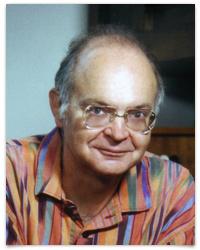
\includegraphics[scale=.5]{images/don_knuth.jpg}
\end{center}
	\caption{Don Knuth, the inventor of \TeX}
	\label{fig:sample}
\end{figure}

\section{Basic Terminology}
As usual the very basic terminology is briefly explained here. Most probably the explanations here only scratch a surface level. More detailed explanations of terminology goes into chapter~\ref{cha:theoretical-background}.

\section{Related Work and Projects}
Here a survey of other work in and around the area of the thesis is given. The reader shall see that the authors of the thesis know their field well and understand the developments there. Furthermore here is a good place to show what relevance the thesis in its field has.

\section{Structure of the Thesis}
%dsflkjas flaksjfl asdfj as lfjldsajflaksdjf sa dfjlasdkfj sadlfjasdklf als dfj l dfsdfsdfn chapter~\ref{cha:used-technologies} (\nameref{cha:used-technologies}) on page~\pageref{cha:used-technologies} we describe the used technologies.
Finally the reader is given a brief description what (s)he can expect in the thesis. Each chapter is introduced with a paragraph roughly describing its content.